\section*{Analyse}
\label{Analyse}
%
%How many dimensions should you use? Plot scree plot
%How well a fit is your solution? Plot Shepard plot and interpret it
%Can you find meaningful dimensions? Label them. 
Analysen foretages på datasættet, som er præsenteret i \autoref{fig:Data} og indeholder sammenligningsdata for vurderingen af ansigtsudtrykkene. 

\begin{figure}[H]
\centering
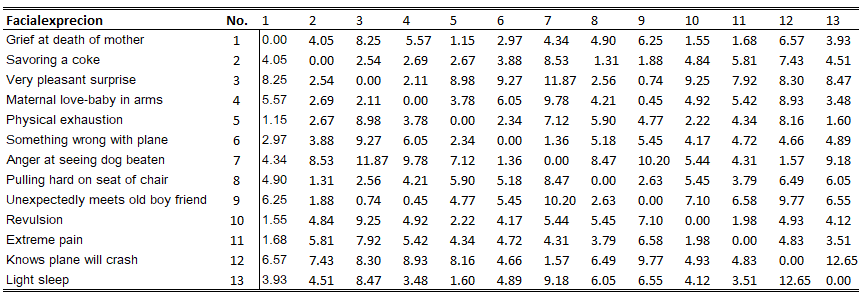
\includegraphics[width = \textwidth]{Figure/Data.PNG} 
\caption{Sammenligning mellem vurderingen af de 13 ansigtsudtryk, hvor 0 indikerer, at ansigtsudtrykkene er vurderet helt ens.}
\label{fig:Data}
\end{figure}

\noindent \autoref{fig:Data} giver ikke et specielt godt overblik over sammenhæng og forskelle mellem vurderingerne af ansigtsudtrykkene. For at få et overblik ønskes det at udføre en \textit{Non-metric MDS}, som beskrevet er beskrevet i \fullref{Metode}. 

\subsection*{Valg af dimensioner}
Første step er at bestemme det optimale antal dimensioner. Måden hvorpå dette gøres, er ved lave et Scree-plot, hvor sammenhængen mellem stress og antal dimensioner kan aflæses ud fra. På \autoref{fig:ScreePlot} er plottet vist. 

\begin{figure}[H]
\centering
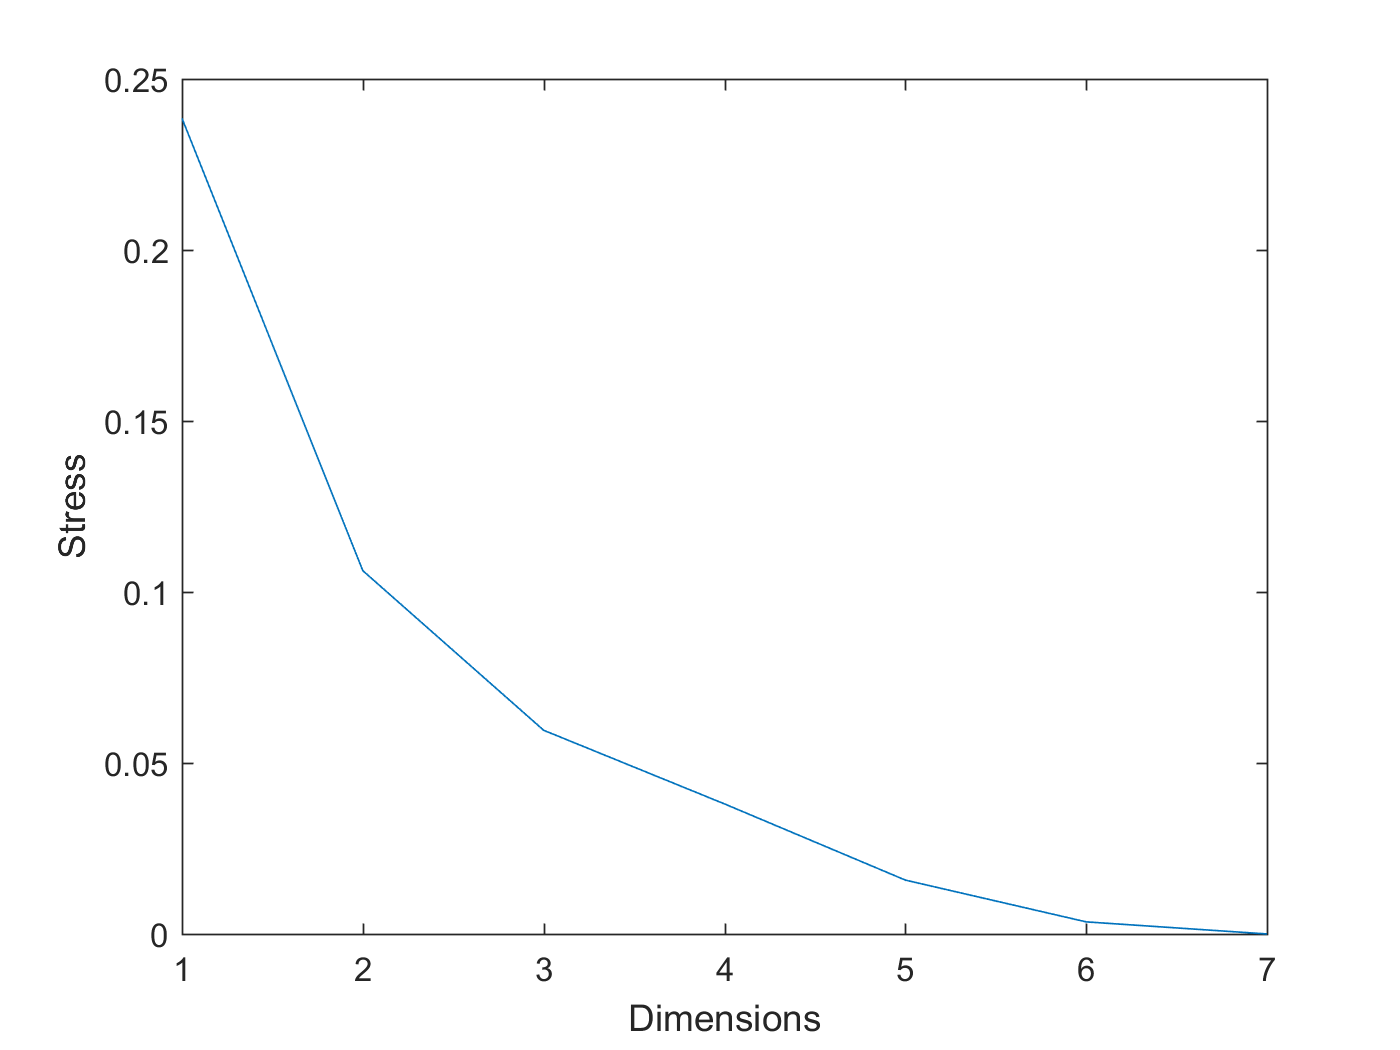
\includegraphics[width = 0.8\textwidth]{Figure/screeplot.png} 
\caption{Scree plot - Forholdet mellem stress og antallet af dimensioner.}
\label{fig:ScreePlot}
\end{figure}

\noindent Scree-plottet har forskellige ``knee''-punkter, som er de steder hvor kurven knækker. Det er ud fra disse punkter at antallet af dimensioner bestemmes, da man her kan se hvor meget stress mindskes ved at øge antallet af dimensioner. 

\noindent Antallet af dimensioner vælges til at være to, der har en stress værdi på 0,1\fxnote{Indsæt præcise værdi.}. Dette antal dimensioner er det første ``knee''-punkt på Scree-plottet på \autoref{fig:ScreePlot} og stress værdien er acceptabel da den svarer til ``fair''. Ydermere mindskes stress betydeligt ved at gå fra en dimension til to, hvor stress ikke mindskes lige så meget ved at gå flere dimensioner op. Det er også vigtigt for valget af dimensioner, at skalaen vil være nemmere at fortolke og arbejde med, hvilket gør sig gældende for to dimensioner.

For at undersøge mere detaljeret, hvor godt disse to dimensioner passer på datasættet laves der et Shepard-plot, som er vist på \autoref{fig:ShepardPlot}.

\begin{figure}[H]
\centering
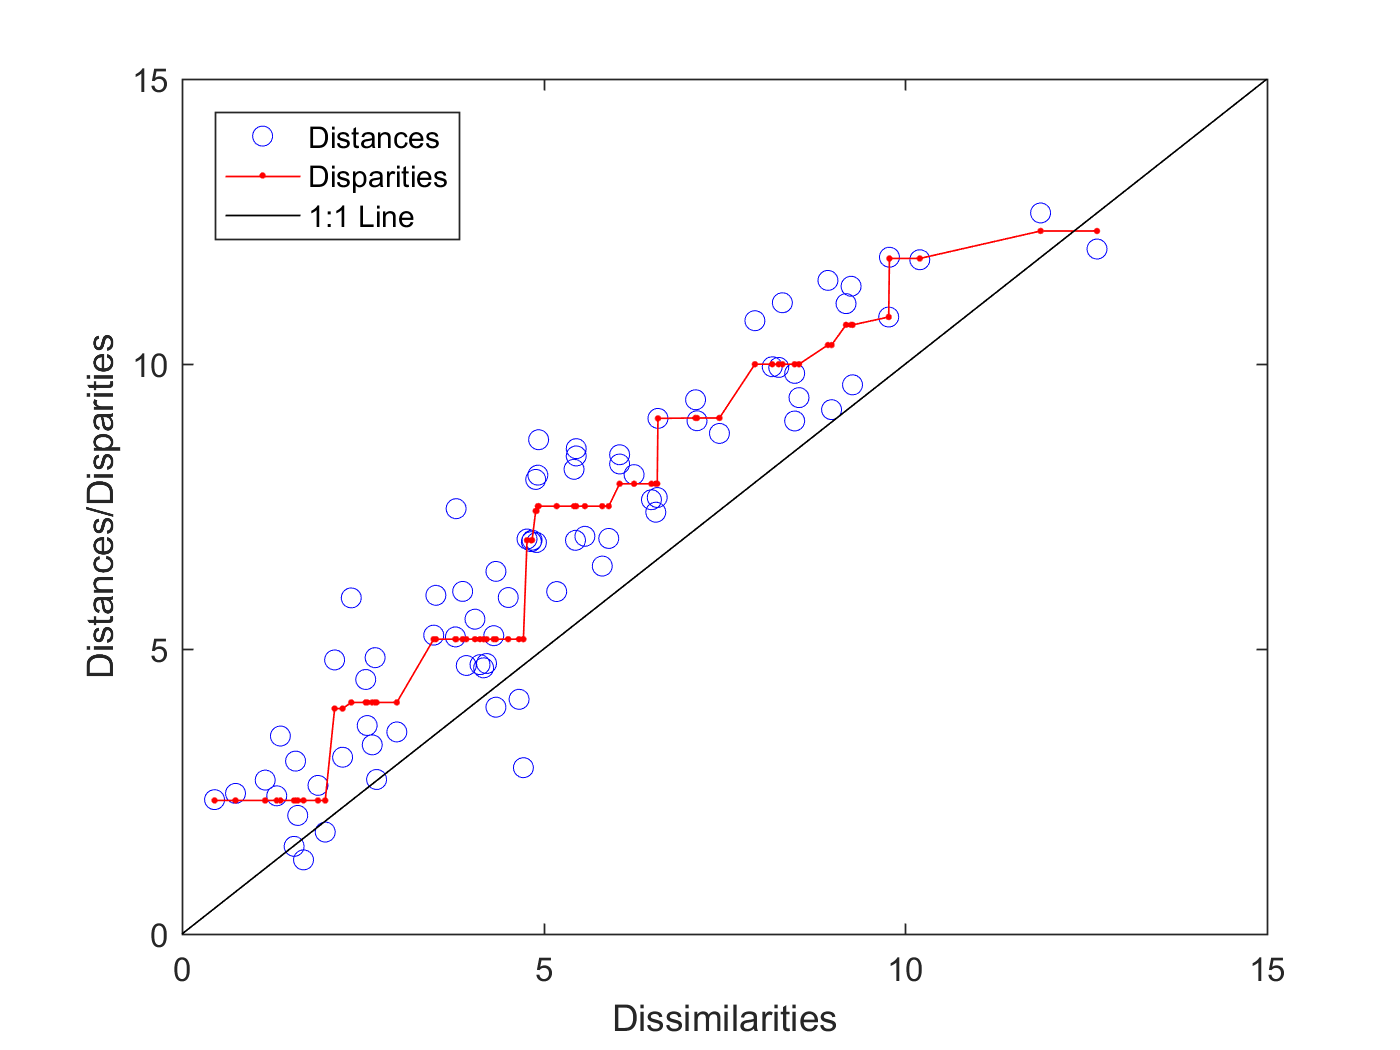
\includegraphics[width = 0.8\textwidth]{Figure/Sheppard_plot.png} 
\caption{Shepard-plot}
\label{fig:ShepardPlot}
\end{figure}

\noindent På Shepard-plottet ses det, at der er nogen afvigelse fra det perfekte fit, som er den sorte linje (1:1 Line). Det vurderes, at den afvigelse, der er fra det perfekte fit, er lille nok til at fortsætte analysen med de valgte 2 dimensioner. 

\subsection*{MDS-plot}
2-dimensionalt non-metric MDS for vurderingen af ansigtsudtrykkene er vist i \autoref{fig:MDS}.  
%
\begin{figure}[H]
\centering
\includegraphics[width =\textwidth]{Figure/MDS_plot} 
\caption{Multidimensional scaling - 2 dimensioner}
\label{fig:MDS}
\end{figure}
%

\noindent Ud fra plottet og placeringen af ansigtsudtrykkene heri, kan det nu undersøges hvilke labels de to dimensioner kan have, som kan give mening i forhold til hvordan ansigtsudtrykkene er placeret. 
\\\\
Dimension 1, som er den vandrette akse (x-aksen) på plottet, kan være \textbf{negativitet}, på engelsk \textbf{Negativity}. Hvis værdien stiger vil personen være mere negativ. Hvis værdien er under nul, vil personen være mere positiv, som vurderes som det modsatte af negativ. 
\\\\
Dimension 2, som er den lodrette akse (y-aksen) på plottet, kan være \textbf{fraværende}, på engelsk \textbf{Absent-minded}. Hvis værdien stiger vil personen være mere fraværende. Hvis værdien er under nul, vil personen være mere tilstedeværende, som vurderes som det modsatte af fraværende. 
\\\\
Det kan ikke undgås at der vil være afvigelser fra de labels der sættes på dimensionerne, da der ved to dimensioner er en stress-værdi på 0,1, som betyder at det det ikke er et perfekt fit ved to dimensioner, og nogle punkter derfor vil være placeret tættere eller længere fra hinanden end den forskel der reelt er.
\\\\
På \autoref{fig:MDSA} er der tilføjet pile i forhold til tolkningen af forskellige parametre.  
%
\begin{figure}[H]
\centering
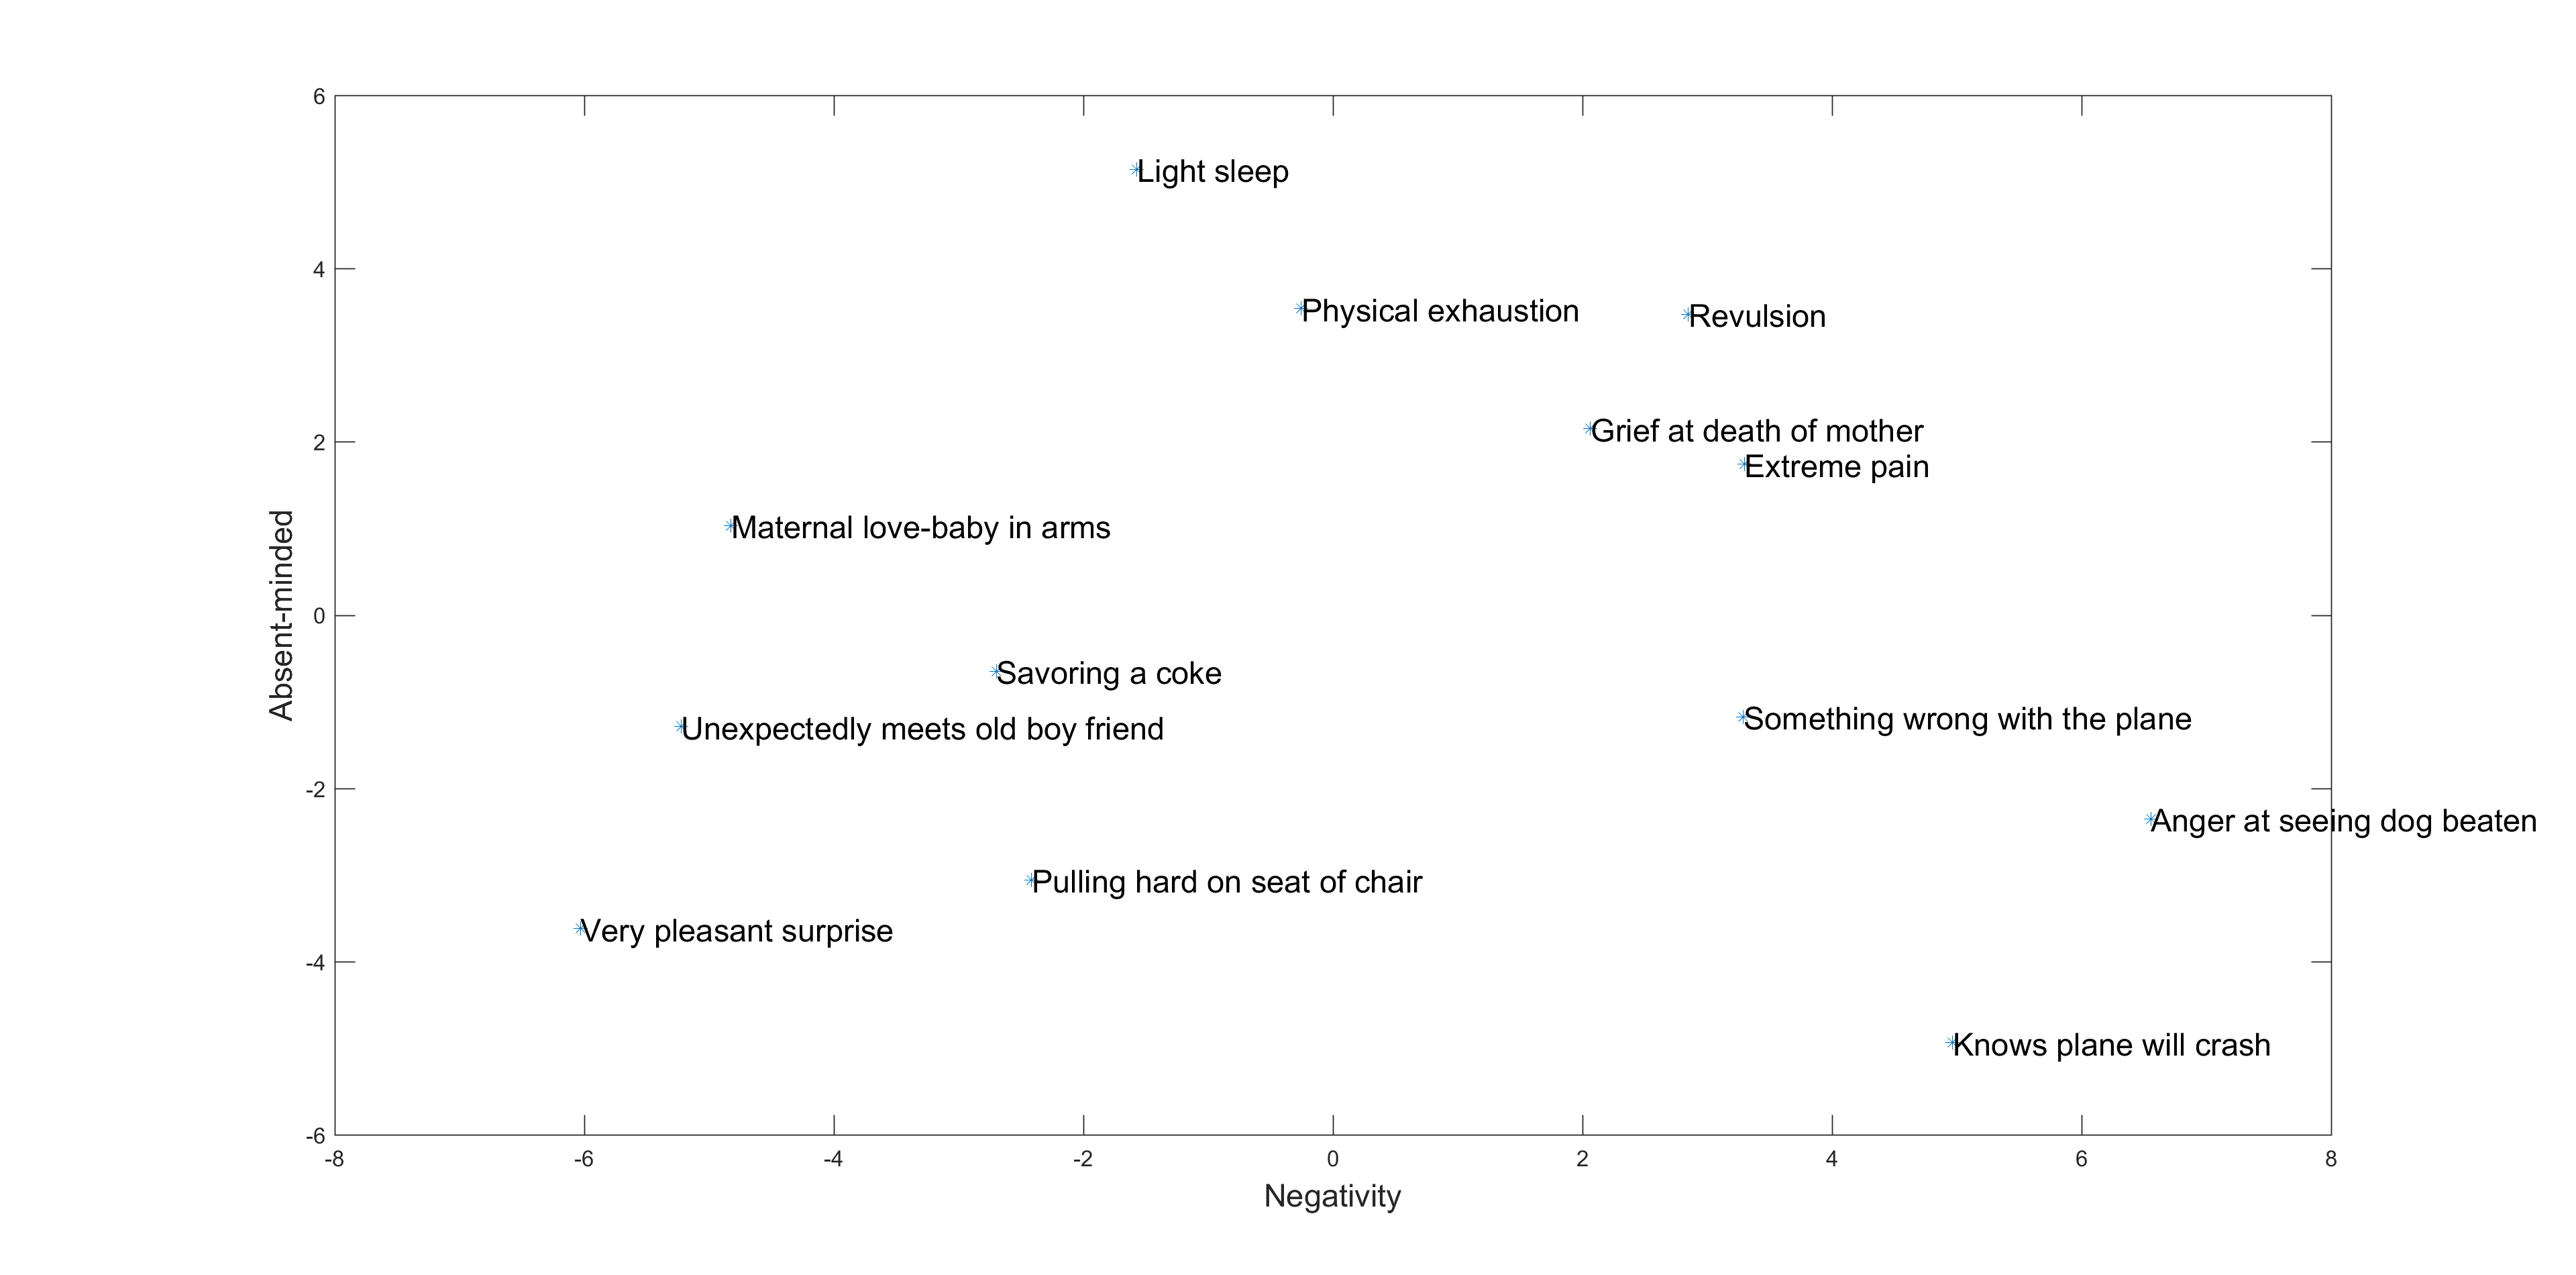
\includegraphics[width =\textwidth]{Figure/mds_plot2.png} 
\caption{Multidimensional scaling - 2 dimensioner, med indsatte vektorer og labels.}
\label{fig:MDSA}
\end{figure}
\noindent
%